\documentclass[10pt]{article}
\usepackage[utf8]{inputenc}
\usepackage[english]{babel}

\usepackage{multicol}

%images insertion
\usepackage{graphicx}
\usepackage{float}
\usepackage{wrapfig}

\usepackage[acronym, automake]{glossaries}
\usepackage[margin=1in]{geometry}
\usepackage{titlesec}
\usepackage{indentfirst}
\usepackage{helvet}
\usepackage{hyperref}
%\RequirePackage[hyperpageref]{backref}

%Bibliography
\usepackage{biblatex}
\addbibresource{bibliography.bib}


\renewcommand{\familydefault}{\sfdefault}
\addtolength{\topmargin}{-0.5cm}
\graphicspath{ {figures/} }
\usepackage[nottoc]{tocbibind}
\usepackage{lmodern,textcomp}
\usepackage{wrapfig}
\titleformat{\chapter}[display]{\normalfont\bfseries}{}{0pt}{\Large}    
\setlength{\emergencystretch}{10pt}
\renewcommand{\arraystretch}{2}


\makeglossaries


\newglossaryentry{framework}{
        name=framework,
        description={Appelé aussi infrastructure logicielle, désigne un ensemble cohérent de composants logiciels structurels, qui sert à créer les fondations ainsi que les grandes lignes de tout ou d’une partie d'un logiciel (architecture)}
    }
\newglossaryentry{MACs}{
        name=MACs,
        description={MACs is the number of Multiply-Accumulates which measures the number of fused Multiplication and Addition operations}
    }
\newglossaryentry{mAP}{
        name=mAP,
        description={ Mean average presition is the metric to measure the accuracy of object detectors like Faster R-CNN, SSD, etc. It is the average of the maximum precisions at different recall values}
    }




\begin{document}
    \begin{titlepage}
        \begin{figure}%
            \begin{minipage}[c]{0.40\linewidth}%
                
\includegraphics[width=\textwidth]{ECN.JPG}
            \end{minipage}
            \hspace{4cm}
            \begin{minipage}[c]{0.30\linewidth}%
                
\includegraphics[width=\textwidth]{logo-aau.png}
            \end{minipage}
            \vspace{2cm}
        \end{figure}%
        \centering
        {\Large Option PRO R \& D 3\textsuperscript{ème} année \par}
        \vspace{1cm}
        {\huge\bfseries study of a localization solution based on the recognition of known objects \par}
        \vspace{1.5cm}
        {\Large\itshape FRERING Laurent  \par}
        {\Large\itshape GONZALEZ-DUQUE Vanessa  \par}
        \vfill
        \begin{minipage}[t]{0.5\textwidth}%
            \centering
            {\bfseries Option teacher:}\\
            {BOURGUIGNON Sebastien}
        \end{minipage}%
        \begin{minipage}[t]{0.5\textwidth}%
            \centering
            {\bfseries Tutor:}\\
            {SERVIÈRES Myriam}
        \end{minipage}%
        \vspace{2cm}
        {Year 2018/2019}
    \end{titlepage}
    

    \pagenumbering{gobble}
    \newpage
    \pagenumbering{arabic}
    
    \section*{ABSTRACT}
    
    In the following work, we first present our analysis of different object detection algorithms, our objective being to select the most relevant for the detection of Nantes' bike-sharing system stations and other urban furniture such as bus or tram stations. Our work is part of a bigger project that aims at implement a mobile augmented-reality application for moving in Nantes. In the second part, we present the results of 7 chosen algorithms applied over our dataset. 
    
    This specific use-case generates several constraints for the algorithms. Indeed, the algorithms have to be run on a mobile device with limited memory processing speed, and the captured images may be of varying qualities. The chosen algorithm should be efficient enough to perform on real time on these devices. \newline
    
    {\itshape \bfseries keywords: Window's analysis, Neuronal Networks, object recognition} 
    \newpage
    
    
    
    \tableofcontents
    
    \newpage
    \section*{Introduction}
    \addcontentsline{toc}{section}{Introduction}

\setlength{\parindent}{10ex} Improving the accuracy and precision of the location delivered by a cell phone is a challenge since 1st May 2000 at midnight, when the Defense Department ended the purposeful degradation of GPS ("Selective Availability" implemented before the first Gulf War), by order of President Bill Clinton.\cite{canales2018navigating}. Since then, GPS became ten times more accurate and more accessible to the civilian population.\footnote{The first commercially-available GPS phone manufactured in 1999 became popular in europe.} GPS integration into mobile devices apps was a success. That's when, problems of signal degradation \footnote{when localization differs a few meters from the real one, due to the disturbances generated by the morphology of the environment and the geometry of the buildings} boost the research area in charge of correcting it.
\begin{figure}[h]
      	\centering
        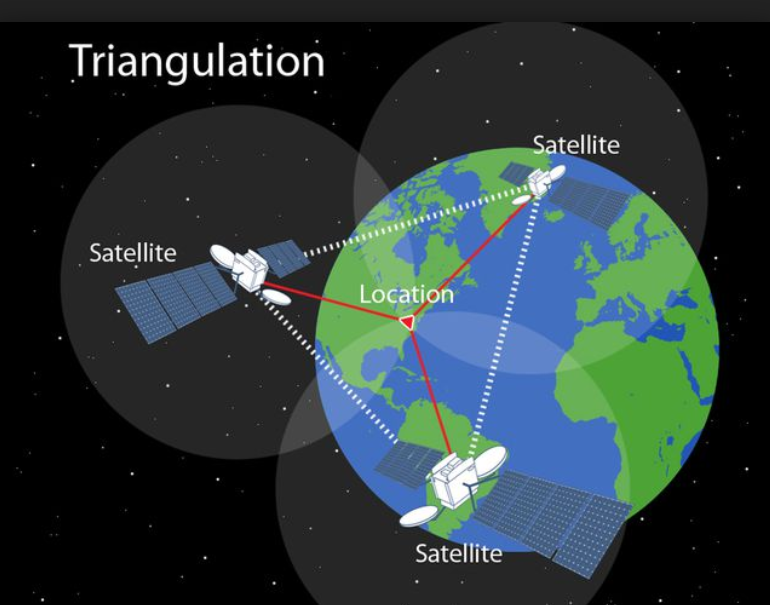
\includegraphics[scale=0.4]{triangulation.PNG}
        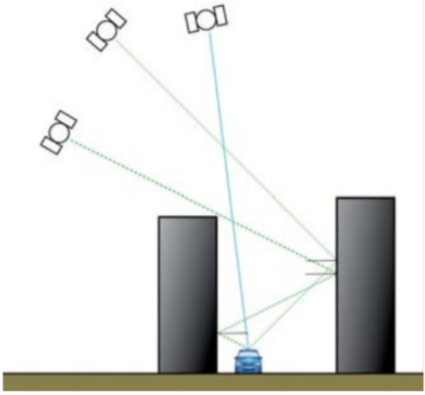
\includegraphics[scale=0.5]{rebota.PNG}
        \caption{Triangulation cited from national geographic? https://www.nationalgeographic.org/photo/triangulation-sized/ and Signal that bounces off buildings from rapport string GROVES ET AL}
\end{figure}



\setlength{\parindent}{0ex}Since 2015, Nicolas ANTIGNY, doctorant à l’IFSTTAR \footnote{Institut Français des Sciences et Technologies, des Transports, de l’Aménagement et des Réseaux}, works in a mobility aid tool for pedestrians in the city, taking advantage of consumer mobile tools of the smartphone type. The goal of the whole project is to provide a mobile augmented-reality application for users to navigate in the city of Nantes.This mobility aid tool would make it possible to visualize, on a mobile terminal, information contained in a Geographic Information System (GIS) during navigation. To do this, it is essential to know the geographical position and the orientation of the terminal at all times and precise positioning (between 10cm and 20cm) of the device, which represents a a real technical challenge. 


One of the obvious solution would be to use GPS-based positioning, but the urban environment comes with different issues making it impossible to achieve a good-enough precision with this technology. For example, measurements taken by the satellites often correspond to the signal that bounces off buildings before returning to the origin (satelite), or gps signal gps' loses.


The approach envisaged consists in designing a hybrid method, based on mutually different methods of computer vision and inertial navigation.  Weighting internal parameters such as the gyrometers, acelerometers and gps datas. An odometry algorithm has been developed, allowing a precise positioning during a displacement of approximately one to two hundred meters \cite{antigny2017pedestrian}. Therefore, it arises the need to recalibrate the global position of the device at this frequency. The solution that was chosen is to use the easily-recognizable street furniture whose global earth coordinates are known \textit{a priori}: "a bicloo station".Nevertheless, it was also the idea of expanding the process to other objects such as bus or tram stations if this concept proves itself successful. From there arises the need to recognize objects in the in the vision brand of the project.


When the bicycle station in corrected detected by visual methods, we proceed to estimate the position of the camera.
Calculating the position and orientation of its optical center related to the projection of the 3D geometric points on a taken image. \cite{Rapport}. \cite{antigny2017pedestrian}\\



\newpage
    \section{Project explanation}
    \subsection{Initial state of the project}
    
In 2016 different object detection algorithms were studied for Hakim CHEIKH \footnote{Élève ingénieur 2ème année de l’école Centrale de Nantes} to solve the "bicloo station detection problem".

The first one was the Viola and Jones detection framework (2001) from Matlab Computer Vision System Toolbox. It was choose for its performance in "STOP signals detection" (\cite{LectureA} ) with a boosting learning method. \footnote{It consists in building a "strong" classifier from a weighted combination of "weak" classifiers, i.e. averaging a better answer than a random draw}. It failed
in 100\% of cases, due to the complexity of the stations and the fact that one must be able to detect these according to several angles of views.

The second studied algorithm was the bag-of-words model (BoW model) that treats image features as words. Visual words are extracted by cutting the visual words according to a regular grid or by using a detection of points of interest.
Then an histogram is build counting the occurrence of similar segments. 
Local descriptors are build with Swift \footnote{(Scale Invariant Features Transform} or Surf\footnote{Speeded Up Robust Features} methods. They are based on detection of points of interest stable to the transformations that an image can undergo (rotation, perspective, ...), generating a vector of 128 dimensions (64 in Surf case). It is important to note that this calculation takes a long time. After visual word extractions, the K-means  clustering algorithm is applied several times with different values of K (dictionary's size).

 
The third studied algorithm allows the machine to learn. It is called, the support vector machine (SVM). It creates a histogram of occurrences of visual words, similar to the BoW, and it estimates the parameters of a a Gaussian kernel doing a cross-validation learning method. 


The last studied algorithm allowed the detection of the object with a searching sliding window, calculating the percentage of match.


The results are positives, 98\% of success. He applied the sift descriptor, then the k-means clustering, the support vector machine and finally the sliding window. Moreover, the calculation time was about 7 minutes per image. What is not at all compatible with the real-time constraint we want to achieve.

    \subsection{Our contribution to the the project}

Currently, the object detection algorithms used to find "Bicloo stations" in a picture were proven precise albeit too time-consuming for a real-time application as is the objective here. Our goal is to find and compare the state-of-the-art algorithms, both the staple and the newer ones, and check if it is possible to detect the street furniture in real-time.\\

Our work was then defined as follow: we have to search for and find new algorithms that were developed recently and that allow for a real-time object detection. These algorithms should be appropriate for our scope, our use-cases being the detection of bicloo station (at first) in a video taken by a pedestrian with a smartphone in hand while moving, and other street furniture after this. 
It is important for us to keep this in mind during the project, as the other street furniture, such as bus and tram stations, contain transparent parts that may not be as easily recognizable as a bicloo station. To summarize, we have to submit a proof of concept comparing different algorithms according to the previously-described use-cases and show how well they perform in real-time.
7 algorithms were compared : SURF descriptors\cite{bay2006surf}, FasterRCNN\cite{FasterRCNN}, YOLOv3\cite{redmon2017yolo9000} and SSD\cite{liu2016ssd} as they are the most famous ones for this kind of application, TinyYOLO\cite{tfjs-yolo-tiny} and TinySSD\cite{wong2018tiny} that are faster versions of previous ones, MaskRCNN\cite{he2017mask} and PeleeNet\cite{wang2018pelee} which are more recent algorithms and the Hifi Skeleton detection algorithm.  \\
% Maybe even more algorithms !

\subsection{Constraints for the choice of the algorithm}

We have different constraints that directly comes from the global project goals. We have to find a way to detect if an element of \emph{a given set of objects} is present in a picture. We also have to detect these objects in \emph{real-time}. As we are concentrating on pretty big street furniture, we can if needed make the reasonable hypothesis that the object is taking a \emph{consequent portion of the picture}. It is also admitted that \emph{we know exactly the shape of the objects}, and even \emph{their 3D models}. We have to be able to detect them \emph{from any angle} and at \emph{different scales}. We also do not know the orientation of the mobile device
% But do we know the intrinsic parameters of the camera ? Either because we suppose that we detect on which phone we are, or because we suppose that a camera calibration is made previously
so we should have an algorithm that is \emph{robust to orientation changes} and somewhat robust to distortion too. As discussed before, the solution will need to perform relatively well when confronted to \emph{known transparent structures}.
Given the scope of the project, it is also required to use open-source solutions as much as possible to avoid legal stops due to property issues.
Finally, the solution should be able to work on \emph{mobile devices} ; it will therefore important to check that the algorithms are not too hardware-dependant and are implementable on such a device.\\


\textbf{Constraints list}

\begin{itemize}
    \item Open-source
    \item Able to run on mobile devices. Low-memory, low-processing power required
    \item Able to run in real-time on mobile devices
    \item Robust to scale, orientation and distorsion changes
    \item Require the smallest and most convenient dataset possible
    \item Perform well when confronted to \emph{known transparent structures} such as bus stations
\end{itemize}

We will also choose algorithms that are widely-used for this type of application, in order to have a basis for comparison.


    \subsection{Task division}
    
% Il faut penser à mettre les liens de tous les datasets cités
\begin{center}
\begin{tabular}{ ||p{3cm}|p{2cm}|p{8cm}||  }
\hline
Task & Time & Difficulties \\
\hline \hline
Chose of algorithms & 2months  & A lot of algorithms, go in many directions, neuronal networks, desition threes, etc  \\
\hline
Table of scores 5x6 & 2 months & Many quantitative and qualitive factors \\
\hline
Understand algorithms & 1months  & Additional information to better understand the work.  \\
\hline
Urban furnitures dataset & 1 week & Private information \\
\hline
installation of a virtual machine & 1 week & Tensorflow instalation requirements, python 3.6 not 3.7 \\
\hline
Dataset modifications & 3 weeks & Tedious task, define one format annotation, CONVERTISEUR DES FORMATS? \\
\hline
Test codes & 4 weeks & I hope all work. Base données 100 images por 10 specific points detection \\
\hline
\end{tabular}\\
\end{center}


    
    \newpage
    \section{State of the art}
    
    \subsection{History}
    \setlength{\parindent}{10ex} Artificial intelligence is used to extract the three-dimensional structure from images with the goal of achieving full scene understanding.
\setlength{\parindent}{0ex}The computational recognition in images has its origins in the 60's. When the pioneer of artificial intelligence, mathematician, computer scientist, and educator of MIT Seymour Aubrey Papert sought to imitate the human visual system \cite{papert1996seymour}.  

Different approaches of computer vision algorithms have their origins in the 70s. The extraction of edges for example, detects sharp changes in image brightness to capture important events and changes in properties of the world.
Others algorithm's solutions as the labeling of lines, the representation of objects as interconnections of smaller structures, and the motion estimation have their origins in these years too \cite{szeliski2010computer}.

In the 80s, the Scale-space theory was formulated. The object recognition was made with a "different scales image databases" of the object, obtained with a Gaussian kernel smooth process. The depth was represented by varying levels of darkness (shading). Some contour models known as snakes searched to delineating an object outline from a possibly noisy 2D image, but the method required knowledge of the desired contour shape beforehand. Others textures and focus algorithms were implemented too. All this methods were based in introducing additional information in order to solve an ill-posed problem or to prevent overfitting (Regularisation) \cite{brooks1999cambrian}.

In the 90s, The photography boom produced different images procedures and different and better quality photos.  For the first time statistical learning techniques were used in practice to recognize faces in images. A set of eigenfaces was generated performing a mathematical process called component analysis (PCA) that use a co-variance matrix on a large set of images that describe different human faces. With PCA, the image to be searched and the images of the database have to have the same dimensions, and need to be previously aligned (the eyes and mouth). This vectors build a new space, with the components that vary. And the new faces will be compared to those already in the space through the Euclidean distance. \cite{turk1991face}. \\
But it was not until 2001 that the first efficient image recognition algorithm was invented by Paul Viola and Michael Jones. Their demo showed faces being detected in real time on a webcam feed.  The distance among the location of eyes, mouth, nose, etc give a vector hand made classifier.  It is trained on a data set of faces, all in the same position, giving a support vector machine. This SVM does the classification, finding the hyperplane that divides the data set in two classes. So, the algorithm was bad to detecting faces in others configurations that the configuration position of the data set \cite{viola2001rapid}.

    
In 2005, Navneet Dalal and Bill Triggs invented Histograms of oriented gradients algorithm using features too. \cite{dalal2005histograms} They represented an image as Matrix of "gradients", that are rows that gives the direction in which each pixel becomes darker. Subsequently, they take subsets of 16 by 16 pixels and they left only the median. This produce a matrix gradient representation of faces. Then they use matrix comparison distance (i.e: euclidean) with a threshold value for determining if a new image is a face.\\

In 2012 the era of depth learning begins. In the ILSVRC-2012-competition, AlexNet's team solve image recognition by using "feature-based" methods, winning by a large margin.\footnote{$$https://www.youtube.com/watch?v=4eIBisqx9_g$$}  These features are obtained using automatic learning techniques (neuronal networks). Although convolutional networks exists since the 90's, they had not been used in this domain due to the high computational demand (GPU) and the huge amount of data needed to train the network \cite{krizhevsky2012imagenet}.

Having all the necessary conditions and rethinking from the beginning the way to detect objects, the team not only uses neural network to classify, but re-propose it as detector. A border (bounding boxes) is assigned and relations between them are established. The objects are detected even if they are partially occluded. This is the beginning of the era of so-called deep learning. Several implementations have been made trying  \textbf{ to optimize of the regions of application of the convolutional network } originated by the output layer’s variable length \cite{HistoryOfObjectDetetion}.

Such solutions originate two approach subdivisions.\\
\begin{figure}[h]
      	\centering
        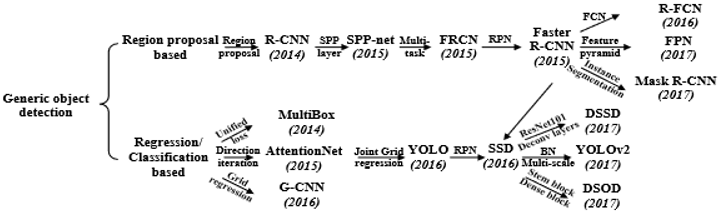
\includegraphics[scale=0.9]{timeline.PNG}
        \caption{Timeline of object detection algorithms \cite{zhao2018object}}
\end{figure}

The first and naive approach was to subdivide in a huge number of regions proposals and then classify each one with a convolutional network. Many algorithms take force, such as R-CNN\footnote{R-CNN: Region Convolutional Neuronal network} \cite{girshick2014rich} , SPP-net\footnote{Spatial Pyramid Pooling in Deep Convolutional Networks for Visual Recognition} \cite{he2014spatial}, Fast R-CNN \url{https://arxiv.org/abs/1504.08083}, Faster R-CNN\cite{ren2015faster},VGGNet\footnote{Visual Geometry Group Network}, R-FCN\footnote{R-FCN: Region-based fully convolutional networks} \cite{dai2016r}, FPN \footnote{FPN: Feature pyramid networks} \cite{lin2017feature} and Mask R-CNN\footnote{Mask-R-CNN: extends Faster R-CNN by adding a branch for predicting an object mask in parallel with the existing branch for bounding box recognition} \cite{he2017mask}. This approach was computational demanding.

The second approach addresses the problem as a regression or classification problem, adopting a unified framework to achieve final results (categories and locations) directly. Among the popular regression algorithms are MultiBox \cite{erhan2014scalable}, bounding box proposal algorithms based on edge recognition \cite{zitnick2014edge}, AttentionNet\cite{yoo2015attentionnet}, G-CNN \cite{najibi2016g}, YOLO\footnote{YOLO: You only looks once} \cite{redmon2016you}, SSD\footnote{single shot detector} \cite{liu2016ssd}, YOLOv2 \footnote{Yolo V2 also called Yolo9000} \cite{redmon2017yolo9000}, DSSD\footnote{DSSD: Deconvolutional single shot detector} \cite{fu2017dssd} and DSOD\footnote{DSOD:  Deeply Supervised Object Detector} \cite{shen2017dsod}.

There exist algorithms like Faster R-CNN that made the bridge between both categories.

\subsection{Recognition algorithms taxonomies and principle explanation }

Object recognition algorithms were regrouped in 5 taxonomies \cite{domingos2015master}: 
\begin{itemize}
    \item Symbolist algorithms: Use of symbols, rules and logic to represent knowledge and draw logical interference 
    \item Bayesians algorithms: Assess the likelihood of occurence of probabilistic inference. As Naive Bayes and Markov. 
    \item Analogizers algorithms: Optimize a function in light of constrains ("going as high as you can, staying on the road"), such as support vectors.
    \item Connectionist algorithms: Recognize and generalize patterns dynamically with matrices of probabilistic weighted neurones, such as neuronal networks.
    \item Evolutionary algorithms: Generate variation and then asses the fitness of each for a given purpose
\end{itemize}

Object detection algorithms were based on segmentation principles (i.e: edge recognition).  That aim at identifying points in a digital image at which the image brightness changes sharply or, more formally, has discontinuities. Until 2011, methods based on features were used. \\ 

 
\subsection{Detection concepts}
When it comes to detecting objects in images, the first thing we must accept is that most of the time they are not centered on the screen, objects have not the same color, they are surrounded by other objects and they may be partially occluded. This is why the detection must be divided into sub-tasks \cite{HistoryOfObjectDetetion}. 

\subsubsection{Bounding box proposal or region proposal}
\setlength{\parindent}{0ex}The first sub task focuses on image segmentation in areas of interest that potentially contain some object. This segmentation process can be made by creating a mask for the foreground (vs. background), by delineating the contour around one or several objects, by giving a semantic label for each pixel in the image, among others heuristic methods.
 
After this segmentation process, a bounding box is represented commonly storing coordinates (4 values in a vector) and the confidence score of how likely the box contains an object (bounding box classifier). Normally the difference between two bounding boxes is usually measured by the L2 distance of their vector representations.
The \textbf{bounding box classifier} can be class-specific if we have one classifier for each object, otherwise, it is called class-agnostic  (one classifier for all classes).

\begin{figure}[h]
      	\centering
        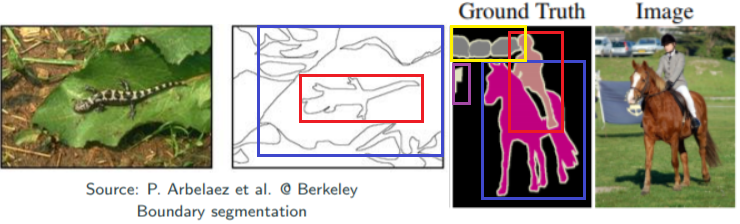
\includegraphics[scale=0.9]{Segmentation.PNG}
        \caption{Modified images with bounding box proposals \cite{Long_2015_CVPR}}
\end{figure}

    
    
    \subsubsection{Bounding box regression}

\begin{wrapfigure}{r}{0.4\textwidth}
  \begin{center}
    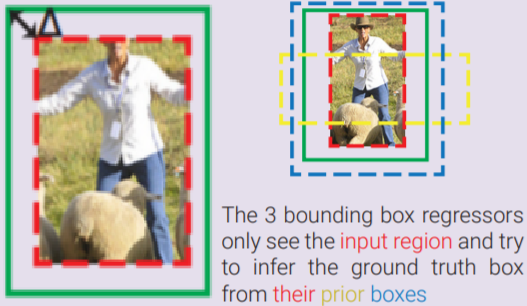
\includegraphics[scale=0.6]{Regression.PNG}
  \end{center}
  \caption{Ground thrue box finded with regression and prior boxes finded ussing matching strategy  \cite{HistoryOfObjectDetetion}}
\end{wrapfigure}

After the segmentation process and the region propositions, it is applied a regression process to find the better box that fit at best the object even if it is partly occluded.

"On regressor can be trained to look at an input region and predict the offset between the input region box and the ground truth box. Bounding box reggressor can be class-specific or class-agnostic too." \cite{HistoryOfObjectDetetion}

    \subsubsection{Box Matching Strategy}
The third part was developed some years before, thinking to improve the bounding box regression detection in bounding box proposals with many objects. 
A box matching strategy was implemented, trying to create \textbf{prior boxes} matching with a \textbf{ground truth box} with highest intertion (IoU= intersection over union) as the SSD, and the FasterRCNN algorithms. \cite{HistoryOfObjectDetetion}\\


\newpage

\subsubsection{Feature pyramid networks}
Feature Pyramid Networks are fast and precise feature extractors designed to generates multiple feature map layers (multi-scale feature maps) with a bottom-up and a top-down pathway with an SSD that makes detection from multiple feature maps.\footnote{With more high-level structures detected, the semantic value for each layer increases.} 

\begin{figure}[H]
  \begin{center}
    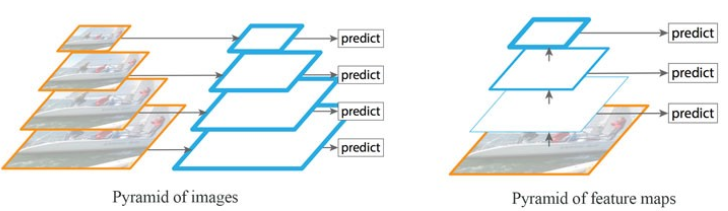
\includegraphics[scale=0.6]{FPN.PNG}
  \end{center}
  \caption{Feature pyramid  \cite{lin2017feature}}
\end{figure}


\subsection{CNN basic concepts}
\subsubsection{Neuronal fully connected networks}
A neuron is an integer number. It is the calculated result of the previous layer times a regularized cost matrix.\footnote{When a  matrix had two or more equals columns, it is not invertible. The added bias assure the inversion of the matrix W because it does not let to exploit the features vectors that are very similar}.\\

\begin{figure}[H]
  \begin{center}
    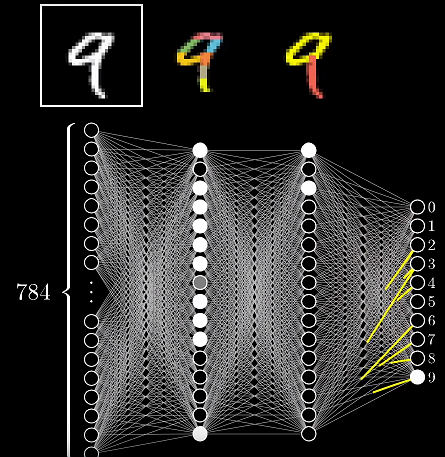
\includegraphics[scale=0.6]{features.PNG}
  \end{center}
  \caption{Feature with number example where the input are the image pixels(781) \cite{NeuronalNetwork}}
\end{figure}


A neuron is active only if the value is bigger than a threshold. If not the neuron is in a "deep dream".
To explain it in a simple way, we will take the example of detection of handwritten numbers. As you can see at left, there are three neurons layers, each one with 16, 16 and 10 neurons (arbitrary chosen). The last layer results in a single active neuron representing the number written in the image, in this case the number 9. The penultimate layer, let's assume that only two neurons are active, one that represents the circle and another that represents the bar that has the number nine. The layer before this, which is the first, has active neurons of the subsections that represent the circle and the subsections that represent the bar. Therefore, the input that is 784 pixels must activate only some specific neurons of the first layer. 

The links among layers are called weights matrix. In this case, there are three weights matrix, one size 784x16 in the first layer, other size 16x16 in the second layer and a third size 16x10 in the last layer. As its name says, this matrix gives a weight (matrix multiplication) to the contribution of each neuron in one layer to every single neuron in the next layer.\\

At the beginning, the network has some default weights. Therefore activates some neurons by default and delivers the prediction of a random number. The training over a numbers write-hand database adjust these weight matrix. 

When the expected result is indicated in a supervised learning (expected active neuron). It modifies the weights that multiply the neurons of the last layer (because they active the expected neuron), increasing some ones and decreasing others. But remember, there are several layers, so another way to activate the expected final neuron is changing the weights in the previous-previous layer that activate certain neurons in the penultimate layer that should or not be active. So, it is a propagate maximization of a cost function, calculated with a back propagation algorithm that became popular in 1986 with Rumelhart et al.\cite{rumelhart1986learning}

A \textbf{feature} is a pattern present in the input (example: A circle and a bar), that  guided the maximization of the cost function that activates x neurons (Negative Gradient equal to Zero). 

The receptive Field is the region of the input image that affects the activation of a feature. ("The circle and the bar"). Generally, a feature in a higher layer has a bigger receptive field,  which allows it to learn to capture a more complex/abstract pattern. 

\subsubsection{Convolutional Network}
% first column
\begin{minipage}[t]{0.5\textwidth}
\begin{figure}[H]
  	\centering
    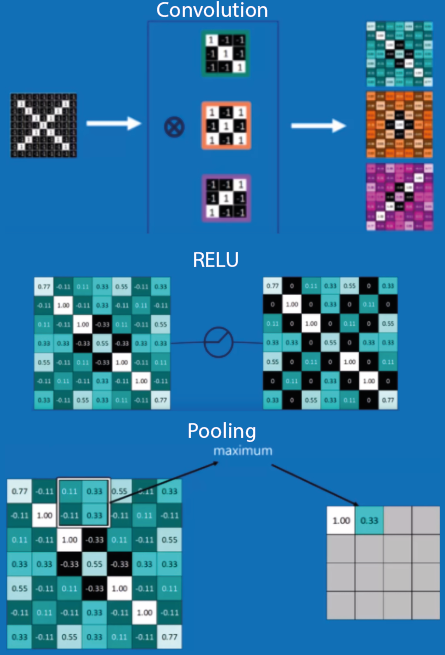
\includegraphics[scale=0.8]{Convolutional.PNG}
    \caption{Operations \cite{ConvolutionalNetwork}}
\end{figure}
\end{minipage}\begin{minipage}[t]{0.5\textwidth}
\begin{figure}[H]
  	\centering
    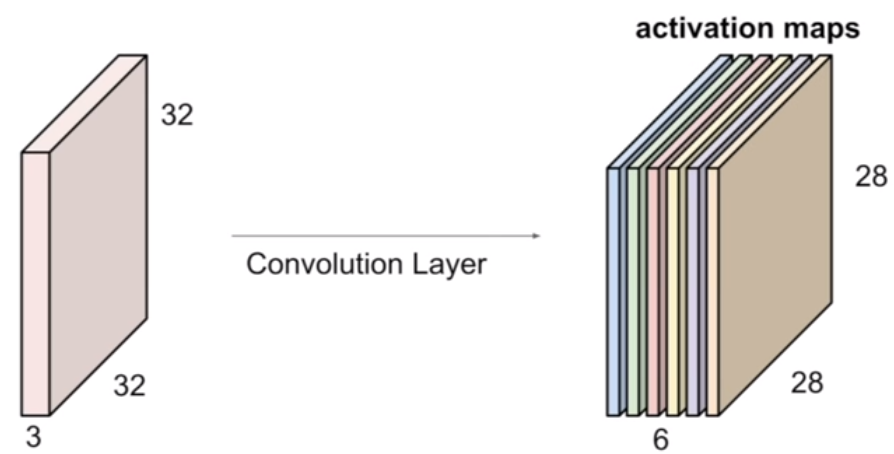
\includegraphics[scale=0.4]{ActivationMap.PNG}
    \caption{Activation Maps produced with convolution \cite{ConvolutionMap}}
\end{figure}
What makes this neural network special are its bi-dimensional neuronal layers. That try to preserve spatial structure. These are obtained through three operations, Convolution, RELU\footnote{ Rectified linear unit is a rectifier or an activation function defined as the positive part of its argument} and Pooling.\\
\textbf{Convolution} consists of taking a filter that detects characteristics, for example a Laplacian that detects contours, and applying it to an image. So an image becomes a stack of filtered images or an stack of \textbf{activation maps} (called also feature volume).\\
\textbf{RELU} consists of making zero the negative values obtained after making the convolution.\\
\textbf{Pooling} consists of choosing subsections of the image and leaving just the bigger ones. So the size decreases. \\
These three operations deliver well defined neuronal layers.
\end{minipage}



\subsection{dataset furniture dataset}
    \href{URL}{ http://homepages.inf.ed.ac.uk/rbf/CVonline/Imagedbase.htm#scene}

    
  Proposér idées de performance: Detection de contours, formes.
  IDÉE: apliquyer une filtre de contours et ces images les inserer au reseau?

    
\newpage    
\section{CNN Algorithms comparation}
The selection of an object detection algorithm for an user case becomes a complicated task when algorithms are very numerous, and additionally, the amount of comparison metrics is very broad. 

Just in the past for years, more than 14 deep neuronal network architectures were presented in the ImageNet challenge\cite{canziani2016analysis}. 
Canziani et all made an analysis of deep neuronal network models and they compare structures in terms of accuracy(mAP), required computational cost (MACs), memory footprint (MB), number of parameters (Millions), inference time\footnote{Inference is the moment when a trained model can say something knowledgeable (predict)} and power consumption.
Additionally, we can be compared them in terms of image processing speed (Fps) and others quantitative and qualitative metrics, as the required size of the tranning dataset for x accurracy.

\begin{figure}[H]
  	\centering
    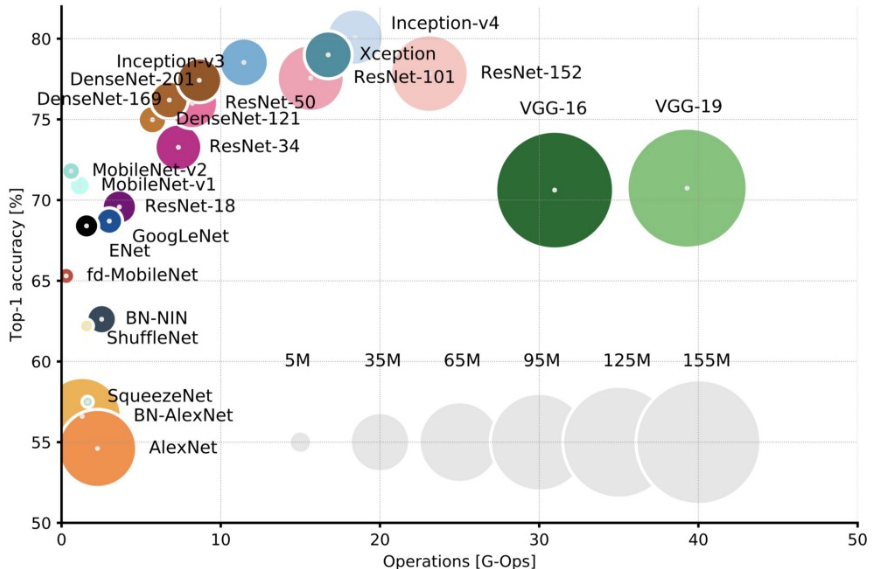
\includegraphics[scale=0.7]{codesComparation.PNG}
    \caption{Top-1 one-crop accuracy versus amount of operations required for a single forward pass \cite{canziani2016analysis}}
\end{figure} 

They key findings of Canziani et all were four. First, they prouve that power consumption is independent of batch size and architecture. Second, the accuracy and inference time are in a hyperbolic relationship. Third, the energy constraint is an upper bound on the maximum achievable accuracy and model complexity. Fourth, the number of operations is a reliable estimate of the inference time. 
This findings help us to define the comparison criteria.

During this section only a summary of 4 parts for each algorithm will be made. First, the main characteristics that made us choose it, including the context, will be exposed. Second, a judged performance score against our criteria will be made. Third, the operation of the algorithm will be briefly summarized. Finally, a reference to the source code will be presented and the requirements for downloading and compiling the code will be listed.\\

\subsection{Tiny-SSD-2018}
1.In the search for algorithms that solve the problem of high computational and memory requirements, we found this algorithm that minimize the size of the neuronal network . Making the algorithm more suitable for embedded devices and real-time operated. Perfect for mobile phones implementation.\cite{wong2018tiny}

The model size fill 2.3MB (26 times smaller than Tiny YOLO) while still achieving an mAP of 61.3\% on VOC 2007 (approximatly 4.2\% higher than Tiny YOLO). The number of filters in each auxiliary convolutional feature layer is optimized to minimize the number of parameters.\\

2. 
From the article of Wong et all, It is presented the accuracy results on VOC 2007. \cite{wong2018tiny} 

\begin{figure}[H]
  	\centering
    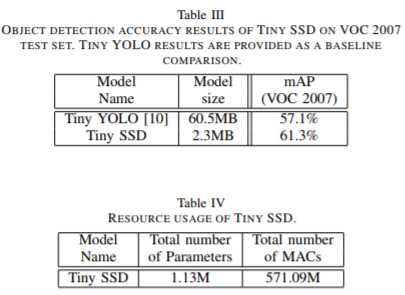
\includegraphics[scale=0.7]{TablaTinySSD.PNG}
    \caption{Comparative table from the TinySDD article over VOC 2007 dataset \cite{wong2018tiny}}
\end{figure} 

The evaluation with our criteria presented positive results in terms of computational cost, memory, speed and accuracy requirements. Additionally, the algorithm is open source. As arguments, it is faster than SSD (59FPS), interesting for the real-time requirements in our usser case. Its computational cost is just 571.09M MACs, value smaller than 3490M MACs on tiny-YOLOv2\cite{wang2018pelee} over the same dataset. The memory spend just arround 2.3MB (model size parameters), and its accurracy is 61.3\% [mAP]. \\


3.It is based on SqueezeDet and SSD. The key idea of SSD, for speed, is the use of a single network detection and no need for region proposals. With some bounding boxes by default, they adjust only the ones with the higher detection's score to match the object and they suppress the others with smaller scores. Another big difference appears on the training. It involves choosing the set of default boxes and scales for detection as well as the elimination strategies for useless boxes (i.e: cutting value). Besides, the train data set must have the ground truth information in the fixed detector outputs (bounding box by default).\\
\begin{figure}[H]
  	\centering
    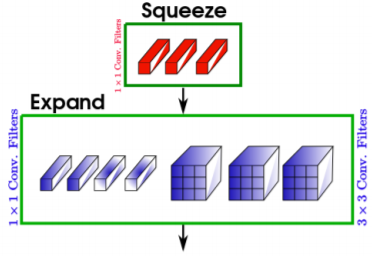
\includegraphics[scale=0.7]{TinySSD.PNG}
    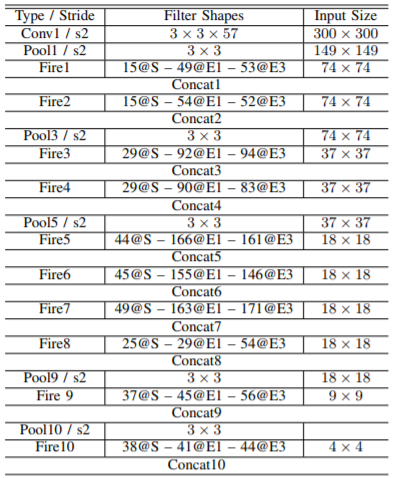
\includegraphics[scale=0.6]{tinySSDarchitecture.PNG}
    \caption{TinySSD architecture \cite{wong2018tiny}}
\end{figure} 

4. We can find the source code in the url \url{https://github.com/lampsonSong/tinySSD}.\\
The proposed Tiny SSD network was trained for 220,000 iterations in the \textbf{Caffe framework} with training batch size of 24. RMSProp was utilized as the training policy with base learning rate set to 0.00001 and gamma = 0.5.\\


\subsection{PeleeNet-2018}

1.Another architecture that try to solve the problem of limited computing power and memory resources is PeleeNet.\cite{wang2018pelee} The comparation with ,\textbf{MobileNet, ShuffleNet and MobileNetV2} presents a high performance algorithm.
In the article, Wang et all said: " It is 1.8 times faster speed than MobileNet and MobileNetV2 on NVIDIA TX2. Meanwhile, PeleeNet is only 66\% of the model size of MobileNet. It achieves 76.4\% mAP on PASCAL VOC2007 and 22.4 mAP on MS COCO dataset at the speed of 23.6 FPS on iPhone 8 and 125 FPS on NVIDIA TX2. The result on COCO outperforms YOLOv2 in consideration of a higher precision, 13.6 times lower computational cost and 11.3 times smaller model size."\\

2.
From the article\cite{wang2018pelee}, it is presented the accuracy results over VOC 2007, over stanford dogs and over ImageNet 2012.  The evaluation with our criteria presented positive results. 

The algorithm is open source. Over Pascal VOC 2007:
It is faster (17.1 FPS on iPhone 6s and 23.6 FPS on iPhone 8) than SSD+MobileNet(16.1 FPS on iPhone 6s and 22.8 FPS on iPhone 8) and than tinyYoloV2 (9.3 FPS on iPhone 6s and \textbf{23.8} FPS on iPhone 8). This is enough for a mobile phone application like ours. 
Its computational cost (1290M MACs) is 13.6 times lower than YoloV2 (17500M MACs), than SSD (34360M MACs) and a bit bigger than SSD+MobileNet(1200M MACs). As the computational cost is low compared to most algorithms, PeleeNet seems interesting for our case.
The model size is very small compared to competing algorithms. It is 11.3 times smaller than for YoloV2 (5.98M parameters against 67.43M parameters), smaller than SSD (34.30M  parameters) and smaller than SSD+MobileNet(6.80M Parameters). According to PeleeNet's paper \cite{wang2018pelee}, the accuracy of Pelee (76.4\%mAPs) is higher than that of TinyYOLOv2 (57.1\%mAPs) by 13.8\%, higher than that of SSD+MobileNet(68\%mAPs) Huang et al. (2016b) by 2.9\% and higher than YoloV2 (69.0\%mAPs). \\

\begin{figure}[H]
  	\centering
    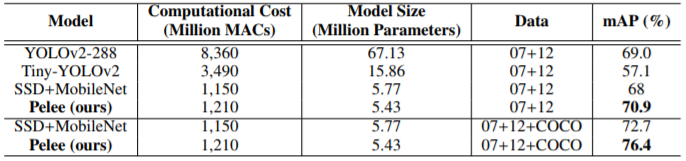
\includegraphics[scale=0.8]{Pelee4.PNG}
    \caption{Results on PASCAL VOC 2007 dataset.\cite{wang2018pelee}}
\end{figure}

\begin{figure}[H]
  	\centering
    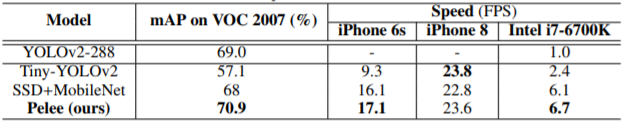
\includegraphics[scale=0.9]{Pelee5.PNG}
    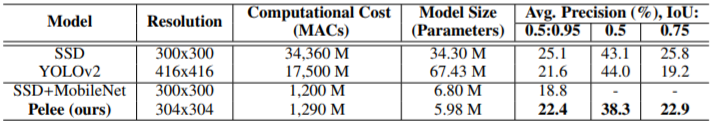
\includegraphics[scale=0.9]{Pelee6.PNG}
    \caption{Speed Comparison on Real Devices.\cite{wang2018pelee}}
\end{figure}

3. It is a real time object detection system on mobile devices. A variant of \textbf{DenseNet}.
The depth-wise separable convolution is heavy to calculate and there is any efficient implementation. Reason why, PeleeNet use a conventional convolution. Combining with a Single Shot multibox Detector (SSD).
\begin{figure}[H]
  	\centering
    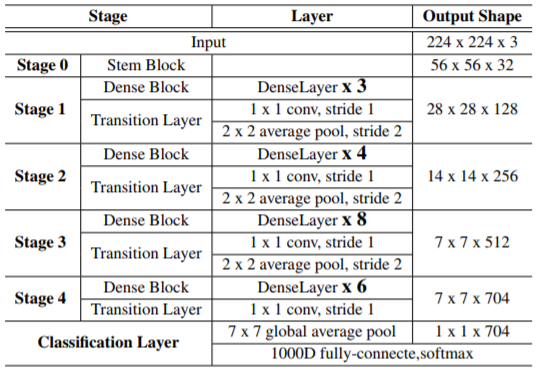
\includegraphics[scale=0.7]{Pelee.PNG}
    \caption{Overview of PeleeNet architecture \cite{wang2018pelee}}
\end{figure}

They made some choices to adapt it on mobile devices: First, there are 24 parameters instead of 64 in the first convolutional layer. Second, the kernel size was changed from 7x7 to 3x3, because ”The accuracy of the model using 1x1 kernels for prediction is almost same as the one of the model using 3x3 kernels. However, 1x1 kernels reduce the computational cost by 21.5\% and the model size by 33.9\% \cite{wang2018pelee}. Third, the number of layers in each dense block is adjusted to meet the computational budget. Others some clever choices are the transitional layer without compression, the Post-activation function, the dynamic bottleneck channels, the Stem block and the Five dense layers (3 more than DenseNet). More information is found in Wang et all parper.\cite{wang2018pelee}

\textbf{Over Stanford Dogs data set}\cite{wang2018pelee}, PeleeNet had similar hyper-parameters used in ResNet on ILSVRC 2012. They randomly adjusted brightness and contrast of training images. \footnote{This new data augmentation approach brings a 0.3\% performance boost.}.The model is trained with a cosine learning rate annealing schedule\footnote{Cosine Learning Rate Annealing means that the learning rate decays with a cosine shape (the learning rate of epoch $t (t <= 120)$ set to $0.5 x lr x (cos(\pi x t/120) + 1)$.}, similar to what is used by Pleiss et al. (2017) and Loshchilov & Hutter (2016)\footnote{MACs is the number of Multiply-Accumulates which measures the number of fused Multiplication and Addition operations.}.\\
\textbf{Over ImageNet ILSVRC 2012 dataset} trained by PyTorch with mini-batch size 256 for 120 epochs. Hyper-parameters are the same as the one used on Stanford Dogs dataset. Trained with a cosine learning rate annealing schedule which starts from 0.1.\\

4. We can find the source code in the url \url{https://github.com/Robert-JunWang/Pelee}.
It is trained with Caffe Jia et al. (2014) with annotation on COCO format. The batch size is set to 32. The learning rate is set to 0.005 initially, then it decreased by a factor of 10 at 80k and 100k iterations,respectively. The total iterations are 120K.


\subsection{YOLO-v3}

1. YOLO is one of the major object detection algorithm around. Recently it lost its place as one of the most accurate algorithms, but it is still widely considered to be among the fastest. This is why it is important in our comparation, as it is one of the staple algorithms, we will discuss it here. YOLOv3\cite{redmon2018yolov3} is a more accurate albeit slower version of YOLOv2, but it is clearly better at detecting small objects.\\

2. It has speed of 20 FPS and 220FPS on it tiny version, interesting for the real-time requirements in our case. However, Yolov2 is faster with 40FPS and 244FPS in its tiny version. 

\begin{figure}[H]
  	\centering
    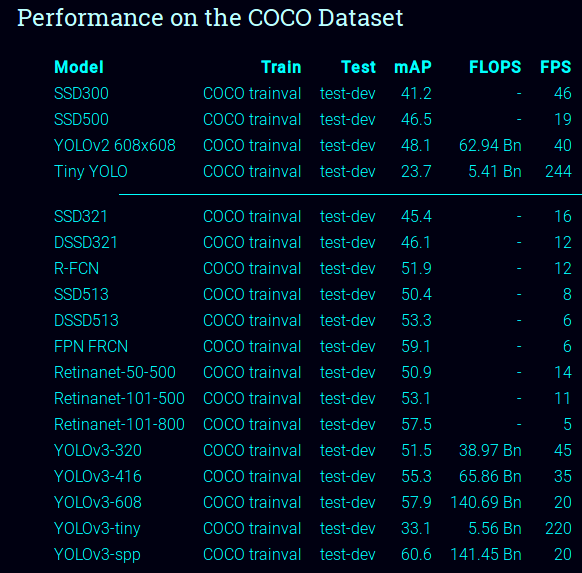
\includegraphics[scale=0.5]{yoloCOCO.png}
    \caption{ Comparation over the COCO dataset\cite{redmon2018yolov3}}
\end{figure}

In accuracy, it performs well, with 60.6\% mAPs and 33.1\% mAPs on its tiny version, better than Yolov2 with 48.1\% mAPs and 23.7\% mAPs its tiny version. The computational cost requirements are small and interesting for us, it has a model size of 141.45 Bn FLOPS and 5.56 Bn FLOPS on its tiny version. a little heavier than YoloV2 with  62.94 Bn FLOPS, and 5.41 Bn FLOPS in its tiny version (Price to pay for the improvement of the accuracy). 

It has low memory requirements perfect for us\footnote{memory requirements:Lower than 500 MB}\\



3. YoloV3 does not struggle, like YoloV2, with small object detections due to the loss of fine-grained features as the layers downsampled the input. It makes detections at three different scales. (With 9 anchor boxes. Three for each scale) The detection kernels have shape of 1 x 1 x (B x (5 \+ C) ), where C is the number of classes and B the number of bounding boxes a cell on the feature map can predict. YoloV3 has important elements like the residual blocks, the skip connections and the upsampling that YoloV2 obviate. Object confidence and class predictions in YOLO v3 are now predicted through logistic regression. This are some of the improvements respect to Yolo v2.


\begin{figure}[H]
  	\centering
    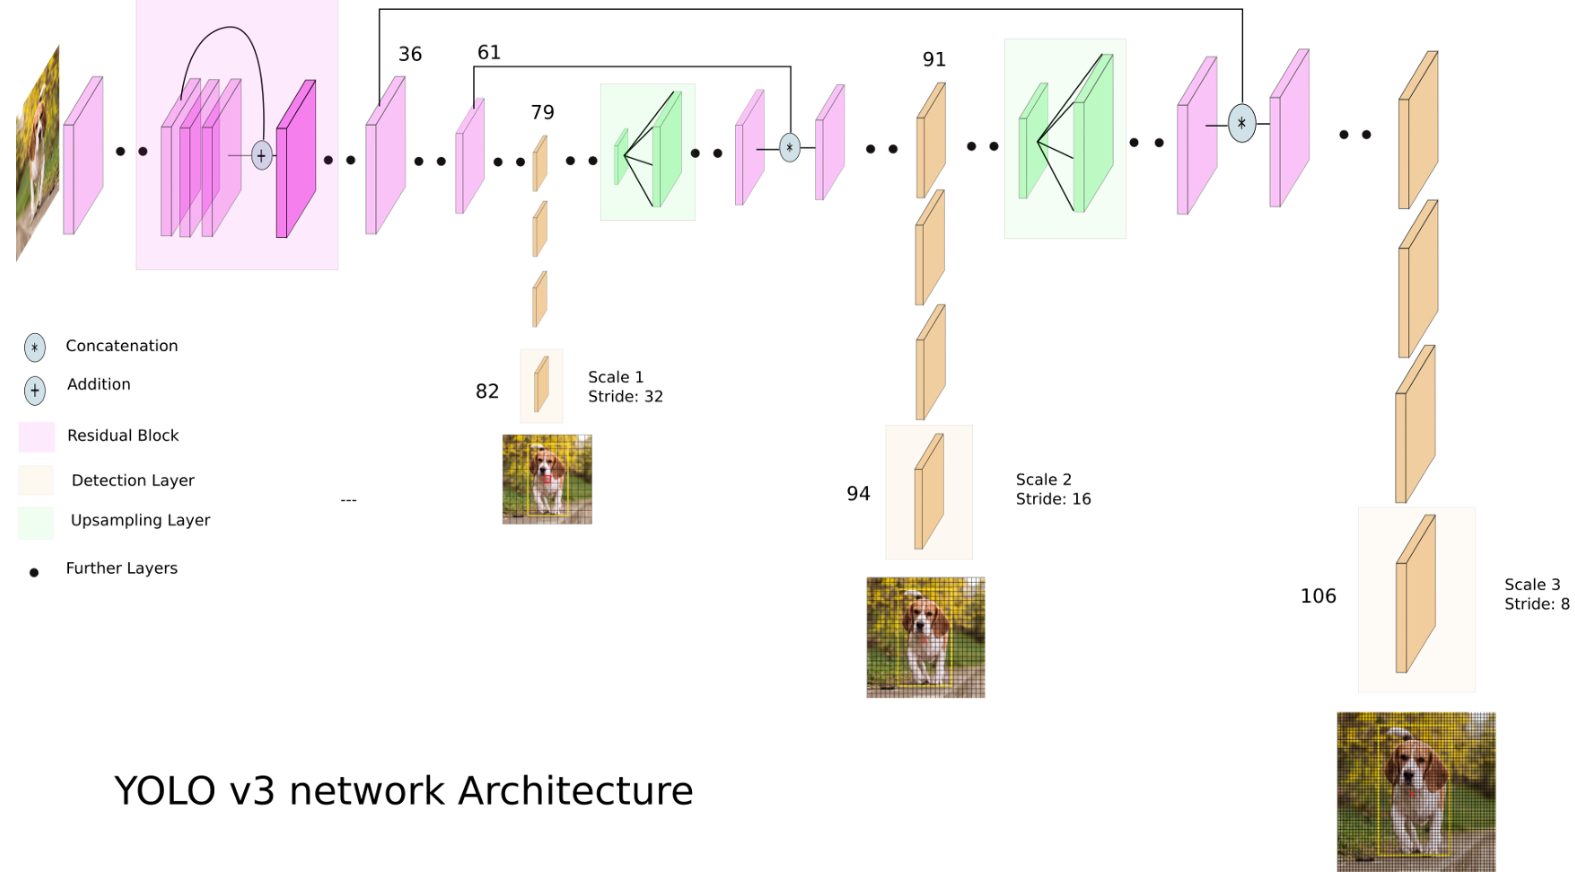
\includegraphics[scale=0.4]{yolov3.PNG}
    \caption{YoloV3 network architecture to YOLO website : \url{https://towardsdatascience.com/yolo-v3-object-detection-53fb7d3bfe6b} accessed on 21th January 2019}
\end{figure}



\subsection{YOLOV2 and Tiny-YOLOV2 - 2017}

1. The possibility of using the source code of this algorithm that does not \textbf{need labelled detection data} makes it an excellent candidate for our use case. Additionally, it can be trained with images of varying sizes, offering an easy trade-off between speed and accuracy. The Tiny version aiming at more FPS by sacrificing precision.\cite{redmon2017yolo9000}. The solution for real time computation is to analyse many windows or boxes in parallel and just once. This implementation is faster due to the 125 parallel analysis.\\

2.
The paper of Redmon et all \cite{redmon2017yolo9000} shows an accuracy of 76.8 mAP on VOC 2007 at a speed of 67 FPS, and 78.6 mAP at 40 FPS. Outperforming state-of-the-art methods like Faster RCNN with ResNet and SSD while still running significantly faster. Result that makes it interesting for us.
The accurracy presented over the same dataset in peleenet article \cite{wang2018pelee} is 57.1\% mAP, at a different speed.

\begin{figure}[H]
  	\centering
    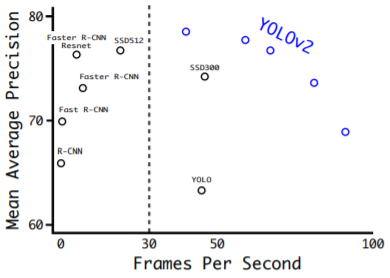
\includegraphics[scale=0.9]{YOLOV2.PNG}
    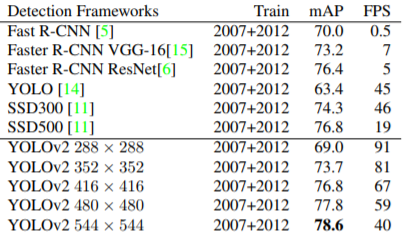
\includegraphics[scale=1]{YOLOV22.PNG}
    \caption{ Accuracy and speed on VOC 2007 from redmon et all \cite{redmon2017yolo9000}}
\end{figure}

On PeleeNet's paper\cite{wang2018pelee} they run at 9.3 FPS the algorithm on iPhone 6, and 23.8 FPS on iPhone 8. The computational cost on PASCAL VOC is 3490 MACs. It demands low memory because its model has just 15.86 Million parameters. Another reason why we consider it would be interesting in mobile applications.\\


3.TinyYOLO-V2 performs CNN and all of his variants.
First, it divides the image into a 13x13 grid. Second, each cells must predict 5 Bounding boxes. Third, each box give us a score of how certainly it is about enclosing some object. The higher the confidence score the fatter the box is. Fourth, only the boxes with a higher score than a threshold are classified. Fifth, a maxpooling process unified the boxes that are sure that are the same object (non-maximal suppression to remove duplication with lower confidence) and again a threshold and the classification process are applied. Sixth, the confidence score for the bounding boxes and the class prediction are combined into one final score that tell us the probability that certain bounding box contain an specific type of object. 

YoloV2 is is the second version of the YOLO with the objective of improving the accuracy significantly while making it faster. 
\begin{figure}[H]
  	\centering
    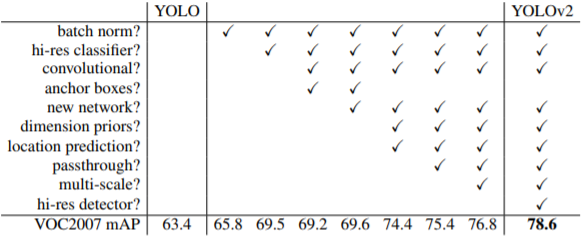
\includegraphics[scale=0.8]{YOLOV23.PNG}
    \caption{ Main improvements \cite{redmon2017yolo9000}}
\end{figure}

The main difference are the addition of batch normalization \cite{ioffe2015batch} in convolution layers\footnote{Batch normalization is used to normalize the inputs of each layer, in order to fight the internal covariance shift problem, also known as the problem of layer adaptation to new distribution in every training step} and the smart chose of bounding box \footnote{Instead of predicting 5 arbitrary boundary boxes, they predict offsets to each of the anchor boxes focused on a specific shape (known a priori). For example, pedestrians have an approximate aspect ratio of 0.41}. Additionally, when we apply the convolutional networks, they give 125 parallel channels for the bricks that contains the data\footnote{Each box has 25 data: Location coordinates x and y, the width and high, the confidence score and the probability distribution over the classes} of the bounding boxes and the class predictions. 

4. Source code in: 
Requirements: COCO format annotations
As tinyYoloV2 can not be trained on any dataset \footnote{ Source code in \url{https://github.com/simo23/tinyYOLOv2}}, we will use tfjs-tiny-yolov2. The source code is \url{https://github.com/justadudewhohacks/tfjs-tiny-yolov2}


\subsection{Mask R-CNN-2018}
1. One of the reasons that made us hesitate to chose this algorithm in the state of the art for our use case was the need for annotated images of the contour of the object for the training phase. This process is not easy to do. However, from the Faster R-CNN repository\cite{matterport_maskrcnn_2017}, they present the possibility of training the network of our own database. The article to which we are directed\cite{MaskRCNNNotations} to understand how annotations are made, explains that sometimes you do not need a million images to train a deep learning model. A \textbf{tiny dataset suffice} if we use the "transfer learning" \footnote{ Transfer learning means that we start the model with a weights file that’s been trained on other dataset. Although this dataset does not contain our class, it helps that the trained weights have already learned a lot of the features common in natural images.} from COCO dataset trainning and if we don't demand  high accuracy from this model. 

The main reasons that make this algorithm interesting for our use are in the first place, the possibility of using our \textbf{own small dataset}. The second reason is the its use for human pose \textbf{keypoints estimation}, since we want to detect keypoints in our object too. The third one is the \textbf{speed of the trainning} step, since Training with ResNet-50-FPN on COCO trainval35k takes 32 hours in a synchronized 8-GPU implementation (0.72s per 16-
image mini-batch). Additionally, it won the COCO 2016 challenge. \\

2. Mask R-CNN is simple to train and adds only a small overhead to Faster R-CNN, running at 5 fps with an accuracy of 62.3\% mAP.\\


3.The goal in this architecture was to develop a
comparably enabling framework for instance segmentation\footnote{Instance segmentation is the classification of objects in categories at the same time of doing the classification of pixels into a fixed set of categories without differentiating object instances (semantic segmentation)} faster and precise.This method extends Faster R-CNN by adding a branch for predicting an \textbf{object mask}\footnote{The mask branch is a small Fully convolutional network applied to each Region of Interest (RoI), that only adds a small computational overhead, enabling a fast system and rapid experimentation.} in parallel with the existing branch for bounding box recognition. 
It works in steps. First, a Region proposal network\footnote{Region proposal network also called light weight neural network} scans all the feature pyramid networks. Second, another neural network scan this regions proposals and generates objects classes(multi-categorical classified), bounding boxes (DeepMask) and masks (SharpMask).\\
\begin{figure}[H]
  	\centering
    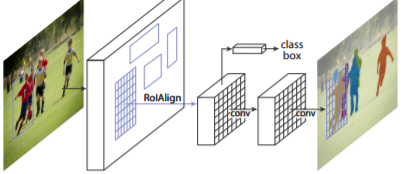
\includegraphics[scale=0.8]{MaskRCNN.PNG}
    \caption{ Main improvements \cite{redmon2017yolo9000}}
\end{figure}



4. Source code in: \url{https://github.com/matterport/Mask_RCNN}
and
\url{https://github.com/facebookresearch/Detectron}
\cite{matterport_maskrcnn_2017}
Requirements:Data set This class provides a consistent way to work with any dataset. It allows you to use new datasets for training without having to change the code of the model. It also supports loading multiple datasets at the same time, which is useful if the objects you want to detect are not all available in one dataset.The images must be in COCO format (json with the COCO API)


\subsection{Faster R-CNN-2015}
1. After FastRCNN, FasterRCNN is the second big improvement on the famous RCNN algorithm \cite{ren2015faster}. Even if it may be considered outdated when compared to more recent algorithm, FasterRCNN is still a go-to algorithm when it comes to object detection, and it is known to be able to perform in real-time. We decided to include it in this study given its excellent track record and as a basis for comparison.\\

2. FasterRCNN is an open-source, CNN algorithm. We can therefore use it, and with a well-chosen dataset it should meet our requirements for robustness.

3.Shaoqing Ren et all.\cite{ren2015faster} proposed an algorithms that learns the regions proposals instead of doing a selective search (method implemented in R-CNN \& Fast R-CNN) that is an slow and time-consuming process.

Similar to Fast R-CNN and R-CNN, the image is provided as an input to a convolutional network which provides a convolutional feature map. Instead of using selective search algorithm on the feature map to identify the region proposals, a separate network is used to predict the region proposals. The predicted region proposals are then reshaped using a RoI pooling layer which is then used to classify the image within the proposed region and predict the offset values for the bounding boxes.

4. Source code in: \url{https://github.com/rbgirshick/py-faster-rcnn}
Dataset annotation format : VOC2007 (standard)



\subsection{SSD}
SSD \cite{liu2016ssd} is a well-known network, usually considered among the fastest and most precise. It is often used in benchmarks and is able to perform in real-time \footnote{\label{gitssd}https://github.com/weiliu89/caffe/tree/ssd}. Testing this algorithm allow for a more comprehensive view, and it is efficient enough to be considered as a possible solution for us. SSD300 and SSD512 used different input image sizes, with SSD300 being faster but less accurate. It is often the better tradeoff.\\

As most of the algorithms here, SSD is an open-source algorithm. The model size is less than 100Mo \ref{gitssd}, which is acceptable in our case. The paper describes the data augmentation and other methods that are used to improve SSD robustness, especially with respect to scale, small objects, and distorsion. \\

SSD's architecture is characterized by the fact that each convolutional layer is used as an input for the classifying neural network. The assumption for the bounding boxes is base on Multibox \cite{szegedy2014scalable} and far more efficient than a random base asumption.

The code is available on Github [\ref{gitssd}].
\newpage


\subsection{SqueezeDet-nov 2017}
S \cite{wu2017squeezedet}
\url{https://github.com/BichenWuUCB/squeezeDet}
\url{https://arxiv.org/abs/1612.01051}


\textbf{Similar algorithms}
\subsection{MobilNet V2}
\subsection{ShuffleNet}
\subsection{NASNat-A}




\newpage    
\section{Weakly-supervised Algorithms}
When there is not available a big amount of notated data, algorithms that detect objects become important.


\subsection{LoANs- Weakly supervised object detection-2015}

!. This algorithm simplifies the process of gathering data for training an object detector. The student-teacher structure is very robust to noise and reaches competitive performance compared to a state-of-theart fully supervised approach. It is simple to create a new dataset, based on a few videos\cite{bartz2018loans}.\\
2. Tabal de caracteristicas?\\

3.The model present the student (localizer) is a model that learns to localize an object, the teacher (assessor) assesses the quality of the localization and provides feedback to the student with the annotations in form of template images that are placed randomly in natural images. The student uses this feedback to learn how to localize objects and is thus entirely supervised by the teacher, as we are using no labels for training the localizer. Localizer is built with the combination of the three modules: Localization Network, Grid Generator, and Image Sampler forms our 

They treat the typical hidden fully connected layer as a convolutional layer. This works because convolutional layers can be thought of as convolving the same fully connected network about the image. 

They add a global max pooling later at the end of this convolutional layer. This is the operator that will "highlight" the area of this final conv layer that has learned the pattern of objects it is trying to classify. Using a threshold on the weights of this global max will ensure a region is significant. Then, they use an algorithm to create a bounding box from this region.

They suggest a new loss function\footnote{A loss function is a measure of how good a prediction model does in terms of being able to predict the expected outcome. A most commonly used method of finding the minimum point of function is “gradient descent”.} that lends itself to an object existing or not. 
They assume a Bernoulli distribution\footnote{Bernoulli distribution is the discrete probability distribution of a random variable which takes the value 1 with probability p and the value 0 with probability q (equal at 1-p)  that is, the probability distribution of any single experiment that asks a yes–no question} for each class which lends itself to multiple logistic regression instead of softmax \footnote{Softmax Regression is a generalization of Logistic Regression that summarizes a 'k' dimensional vector of arbitrary values to a 'k' dimensional vector of values bounded in the range (0, 1). There are thresholding functions. In Logistic Regression we assume that the labels are binary (0 or 1). However, Softmax Regression allows one to handle classes.}.


4. 
Code LOANS:  15 Nov 2018
https://arxiv.org/pdf/1811.05773.pdf
https://github.com/Bartzi/loans 


\subsection{Video Object detection-2017}
1. According to Prest et all \cite{VideoDetection} this method trains object detectors from real world web videos with the only known a priori that images contain the target class instead of using annotated images. The main flaw is that a detector trained on poor-quality web videos does not perform well on still good-quality images. This is not a real problem for us, as the end goal is to detect objects on video flux anyway. This approach could help us a lot, as we have only a very limited set of Bicloo stations images, and it would be easier to use videos shot in Nantes than annotating hundreds of pictures.\\

Comparations are made with a recent weakly supervised method for learning from images..\\

2.
\begin{tabular}{ ||p{3cm}|p{1cm}|p{1cm}|p{8cm}||  }
\hline
Characteristic & Weight & Score & Reason \\
\hline
METRICS?	&0.8 &  &  \\
\hline
Robust to orientation  and distortion	&0.8 &  &  \\
\hline
Quantity of annotated data? &0.7	& & \\
\hline
Robust to size of object (scale) (2 mts distance) &	0.5	& & \\
\hline
Trasparent structures?	&0.4& & \\		
\hline
Robust to texture & & & \\
\end{tabular}\\

3.

4. Source code in: \url{https://github.com/rbgirshick/py-faster-rcnn}.\\
Requirements: The FC CNN layer requires a fixed-size (e.g., 227×227) input image. That is computational dependent. Features are stored on the disk  and training is expensive in space and time. 

\subsection{Skeleton detection-2018}
Everything here is according to \cite{HifiSkeleton}.

Object skeletons are defined as the medial axis of foreground objects surrounded by closed boundaries [Blum, 1967]. Skeletons can notably be used in shape-based image retrieval, which could be useful in our case. This method of skeleton detection is very recent and seems particularly efficient. The code is available at \url{http://mmcheng.net/hifi/}
    
    \begin{figure}[H]
  	\centering
    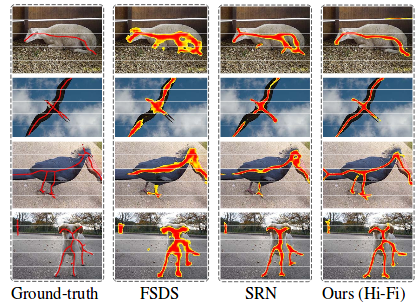
\includegraphics[scale=0.8]{HifiSkeleton.png}
    \caption{Representative detection results. Hi-fi skeletons are more continuous and thinner than others.}
\end{figure}




















\textbf{Comparisons with others algorithms over the same dataset}\\


\section{Benchmarks and comparison between the algorithms}

We first take a look at the benchmark tables provided by YOLO creator Joseph Redmon on his website : 

\begin{figure}[H]
  	\centering
    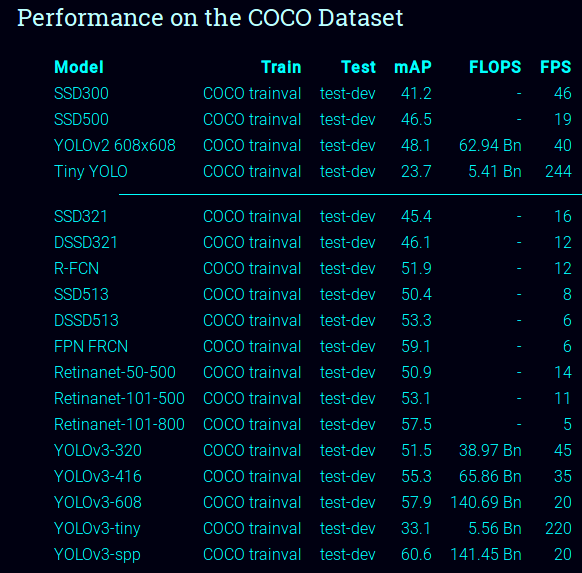
\includegraphics[scale=0.4]{yoloCOCO.png}
    \caption{Comparison of accuracy and speed according to YOLO website : \url{https://pjreddie.com/darknet/yolo/} accessed on 14th January 2019}
\end{figure}

According to Wang et all \cite{wang2018pelee}, we also have the following results :

\begin{figure}[H]
  	\centering
    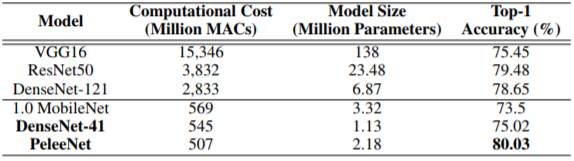
\includegraphics[scale=0.8]{Pelee2.PNG}
    \caption{Results on Stanford Dogs.}
\end{figure}

\begin{figure}[H]
  	\centering
    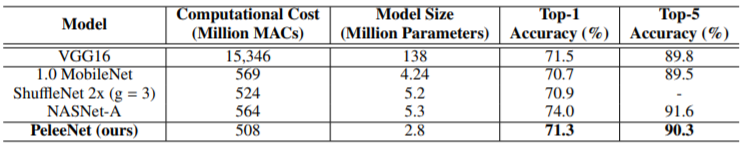
\includegraphics[scale=0.8]{Pelee3.PNG}
    \caption{Results on ImageNet ILSVRC 2012.}
\end{figure}

\begin{figure}[H]
  	\centering
    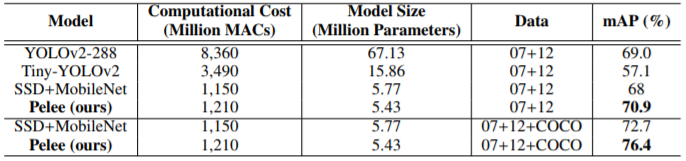
\includegraphics[scale=0.8]{Pelee4.PNG}
    \caption{Results on PASCAL VOC 2007 dataset.}
\end{figure}

\textbf{Speed Comparison}\\
\begin{figure}[H]
  	\centering
    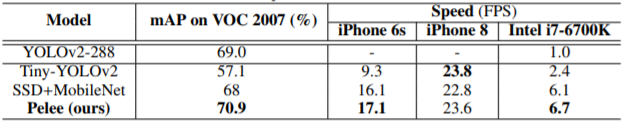
\includegraphics[scale=0.9]{Pelee5.PNG}
    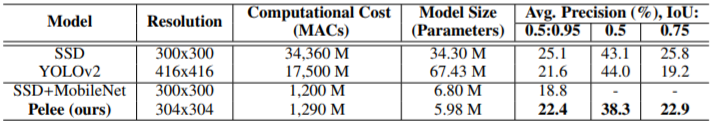
\includegraphics[scale=0.9]{Pelee6.PNG}
    \caption{Speed on Real Devices.}
\end{figure}


\newpage    
\section{Choice of the considered solutions}

In order to select the algorithms we are going to compare in the future, we will use the results of the different benchmarks given before and other, more qualitative criterions.

First of all, all the considered solutions have to be open-source. We will also implement the staple algorithms such as Faster-RCNN, YOLO and SSD in order to have a basis for comparison. We then want to try and use promising algorithms according to their papers and the benchmarks. We will therefore implement TinyYolo which is derived from the widely-used YOLO and designed for real-time application, and PeleeNet which although new and not very well-known seems promising for our use-case. TinySSD is also interesting as it was designed specifically to have a very small model size and to work in real-time.


     textured or non-textured
    Comparison of the sensibility based on a benchmark
    Quantity and type of data needed
    type of object detection
    Memory size
    
    
    fill what we know
    
    
    End January : Comparison table based on criterions + report 
    
    %Tableau récapitulatif de tous les algos, pour comparer facilement. Ici il faudra remplir le tableau qualitativement, avec des '+' ou des '-' par exemple, ou avec une note sur 5 par exemple. Le but c'est surtout d'avoir un comparatif facilement accessible.
    
    \begin{tabular}{ ||p{1.8cm}||p{1cm}|p{1cm}|p{1.8cm}|p{1.5cm}|p{1cm}|p{1.5cm}|p{1.5cm}|p{1.8cm}||  }
\hline
Criterion & SURF & Yolov3 & FasterRCNN & TinyYolo & SSD & TinySSD & PeleeNet & HifiSkeleton\\
\hline
Open-source & & & & & & & & \\
\hline
Robust to scale, orientation, distorsion & & & & & & & & \\
\hline
Quantity of data necessary & & & & & & & & \\
\hline
Formatting of data & & & & & & & & \\
\hline
Performance in real-time & & & & & & & &  \\
\hline
Performance for transparent objects & & & & & & & &  \\
\hline
Computer requirements & & & & & & & & \\
\end{tabular}\\

Evaluation scale :

Question : concerning all the deep-learning algorithms, isn't the robustness just managed using data augmentation? % http://wiki.fast.ai/index.php/Over-fitting#Data_augmentation

Similarly, the quantity of data may be less of a problem if we succeed at extracting data from video. Such tools already exist : https://youtu.be/3BcrK0O1kb4
Or the paper \cite{VideoDetection}

Moreover, concerning the type of data annotation, there are several tools and converters available. 

Very strong tool for annotation : https://github.com/opencv/cvat
Converter : https://github.com/opencv/cvat/pull/9



    \section{Implementation of the different methods and comparison based on our use-cases}
Table type:\\
2. 
\begin{tabular}{ ||p{3cm}|p{1cm}|p{1cm}|p{9cm}||  }
\hline
Characteristic & Weight & Score & Reason \\
\hline
open-source &1& &Yes\\
\hline
real-time	&1 &	&Faster that SSD?\\
\hline
Not heavy and low processor	&0.9 & &Computational cost on PASCAL VOC 2007: 571.09M MACs\\
\hline
Low memory	&0.9& &Model size: 2.3MB \\
\hline
Accuracy	&0.85	&  &mAP: 61.3\% \\
\hline
Robust to orientation  and distortion	&0.8 & & \\
\hline
Quantity of annotated data? &0.7 & & \\
\hline
Robust to size of object (scale) (2 mts distance) &	0.5	& & \\
\hline
Transparent structures?	&0.4& & \\		
\hline
Robust to texture & & & \\
\hline
\end{tabular}\\ 
    \section{Conclusion}
    
    \newpage
    \printbibliography
    
    
    \newpage
    \listoftables
    \listoffigures
    \clearpage
    
    \printglossaries
\end{document}
